\documentclass[tekniskrapport/tech.tex]{subfiles}

\begin{document}

\section{Kommunikationsmodul}
Kommunikationsmodulen styr bilen och kommunicerar med fjärrklienten.
Sensorvärden från sensormodulen tolkas av kommunikationsmodulen som därefter
skickar felvärden till styrmodulen.

Bildbehandling utförs av kommunikationsmodulen för att
avgöra bilens position i vägfilen och upptäcka stopplinjer. Med hjälp av
kamerans bilder på vägen skapas ett felvärde som kan användas för att justera
taxins riktning.

Kommunikation med fjärrklienten sköts av kommunikationsmodulen för
att skicka sensorvärden och annan relevant information. Modulen tar
även emot uppdrag.

Autonomitet utförs av kommunikationsmodulen för att utföra uppdraget.
Kommunikationsmodulen hämtar sensordata från sensormodulen och bildbehandlar
kamerabilderna för att utföra beslut i realtid. Besluten skickas i form av fel-
och styrvärden till styrmodulen.

Kommunikationsmodulens program är skriven i både C och C++. Bildbehandlingen är
skriven i C++ medan resten av programmet är implementerad med C. De olika
delarna kompileras separat och länkas sedan ihop med kompilatorn för C++.
Programmet består av tre trådar; en huvudtråd som hanterar uppdrag och
bildbehandlar, samt en tråd som sköter kommunikation via SPI och en som svarar
på kommandon från fjärrklienten via TCP/IP. SPI:n och servern sköts i separata
trådar eftersom de väntar mycket och blockerar den nuvarande tråden.


\subsection{Hårdvaruimplementation} 
% TODO

\subsection{Programstruktur}
Programmet på kommandomodulen består av följande filer

\begin{labeling}{wwwwwwwwww}
    \item[server.c] Server som anropar kommandofunktioner vid förfrågan från
        klient från separat tråd.
	\item[spi.c] Lågnivåfunktioner för SPI.
    \item[bus.c] Hantering av SPI-buss, utför kommandon på bussen och anropar
        signalhanterare från separat tråd.
    \item[ip/img\_proc.cpp] Bildbehandling med OpenCV.
    \item[objective.c] Utförarande av uppdrag.
    \item[main.c] Huvudloop och implementation av signalhanterare för buss och
        server.
\end{labeling}

\paragraph{Huvudtråden} startar servern och busshanteraren. Därefter startar
den huvudloopen som antingen tar styrvärden utifrån användarens kommandon via
servern eller från uppdragshanteraren med hjälp av bildbehandling. Därefter schemaläggs
skrivning av de nya styrvärdena till styrmodulen. Dessutom schemaläggs hämtning
av sensorvärden från sensorerna.

\paragraph{Servern} erhåller en sockel för nya anslutningar och en för att
skicka och ta emot meddelanden för en aktiv anslutning. Servern kan därmed
endast erhålla en anslutning i taget. Anslutningssockeln är bunden till en port
mellan 9000 och 9100. När en anslutning förfrågas eller om ett meddelande tas
emot väcks servern och accepterar eller tar emot meddelande. Om en
anslutningsförfrågan tas emot skapas en ny sockel för meddelanden och
överskrider den tidigare sockeln om den finns. Om ett meddelande med ett
giltigt kommando tas emot anropas kommandots funktion som utför sin handling
och genererar ett svarsmeddelande som servern sedan vidarebefogar till
klienten. Därefter sover servern igen tills en ny förfrågan tas emot.

\paragraph{Busshanteraren} fungerar på liknande sätt som servern. Den sover
tills en förfrågan sker. Förfrågningarna kommer däremot från andra trådar i
programmet istället för klienten. Om flera förfrågningar sker innan servern har
utfört den nuvarande kommer de nya meddelandena köas i sockeln av
operativsystemet. Det finns dock ingen sockel att köa förfrågningar i för
busshanteraren. Därför har en länkad lista implementerats för att kunna erhålla
flera förfrågningar. När en förfrågan sker läggs den sist i kön och
busshanteraren väcks om den sover. Om kön redan innehåller en förfrågan med
samma kommandotyp ersätts den med den nya förfrågan. Busshanteraren utför
därefter förfrågan via SPI och om kommandot gick igenom anropas
signalhanteraren för det kommandot. Om kommandot inte gick igenom läggs
kommandot sist i kön om ett nyare förfrågan av samma typ inte redan finns i
kön. Annars kastas den äldre förfrågan bort.

\subsection{Bildbehandling}
% TODO

\paragraph{Upptäkt av linjer}

\paragraph{Tolkning av linjer}

\subsection{Uppdrag}

\begin{wrapfigure}{r}{0.3\linewidth}
    \begin{center}
        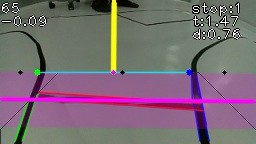
\includegraphics[width=\linewidth]{tekniskrapport/figures/opencv.jpg}
    \end{center}
    \caption{Klassificering och tolkning av linjer från kamera.}
\end{wrapfigure}

\subsubsection{Uppdrag} \label{sec:comm-mission}
% TODO
För att utföra uppdraget kommer en kö av kommandon tas emot från fjärrklienten.
När uppdraget börjar kör taxin framåt och följer filen med hjälp av
bildbehandling och reglering. Inför varje stopplinje tas ett kommando från kön
och utförs. Om ett hinder upptäcks under uppdraget kommer bilen att stanna
tills hindret har försvunnit eller eventuellt passera hindret. När ett visst
antal stopplinjer har passerats och kön är tom är uppdraget avklarat. Nedan är
en lista av alla möjliga kommandon hur de utförs.
\begin{labeling}{wwww}
    \item[\commIgnore] Kör förbi stopplinjen utan att stanna.
    \item[\commStop] Stanna framför stopplinjen, fortsätt efter några sekunder
    om kön inte är tom.
    \item[\commPark] Parkera i fickan till höger efter stopplinjen, lämna
    parkeringen och fortsätt efter några sekunder om kön inte är tom.
    \item[\commEnter] Sväng höger in i rondellen och hitta rondellens körfil.
    \item[\commContinue] Kör förbi stopplinje och håll till vänster.
    \item[\commExit] Sväng höger ut ur rondellen och hitta körfilen.
\end{labeling}

\end{document}
